\section{Design}
\subsection{Overview}
The goal of our dynamic heap resizer is to adjust the size of the primary managed heap (H1) at runtime, based on the total CPU cycles lost to the concurrent GC threads plus STW pauses versus I/O delays ,aiming to improve performance within a fixed DRAM budget. In our setup, the JVM uses TeraHeap, where H1 resides in DRAM and H2 is memory-mapped to an NVMe SSD, with the Linux page cache serving as the cache for H2. Unlike static DRAM division, this approach dynamically changes the size of H1 without requiring any modifications to the application itself.

Operations within H1 are mainly impacted by garbage collection (GC) overhead. Increasing H1 provides more space for new objects, reducing memory pressure and thus decreasing GC frequency and pause times, thereby preserving compute cycles for mutator threads. However, allocating more DRAM to H1 also reduces the memory available for the page cache of H2, potentially increasing I/O cost due to more frequent and expensive page faults when accessing SSD-resident data.

To balance these trade-offs, the dynamic resizer collects the totall lost compute cycles from concurrent GC thread CPU usage and STW pauses, and I/O metrics at regular sampling intervals. Using these insights, the system determines how to partition DRAM between H1 and the page cache for H2 by deciding whether to grow or shrink H1. When H1 is shrunk, the freed physical memory is reclaimed by the operating system and becomes available for the H2 page cache.

Because resizing decisions do not have immediate effects – for example, growing H1 reclaims pages from the H2 page cache only when the JVM accesses them, and shrinking H1 frees memory for H2 cache only after page faults trigger it – the Dynamic Heap Resizer incorporates a finite state machine (FSM) to manage adaptation safely. This FSM introduces wait states after each resizing action, allowing the system to observe the impact before making further changes, and includes direct state transitions to improve responsiveness and avoid delays. Figure \ref{fig:dynamic_heap_resizer} illustrates the architecture and workflow of the Dynamic Heap Resizer within our setup.


Overall, by dynamically adapting the size of H1 at runtime, our system enables TeraHeap to maintain low GC overheads during memory-intensive phases while ensuring sufficient DRAM page cache capacity for I/O-heavy phases, leading to improved performance without modifying application logic or the underlying hybrid heap architecture.

\begin{figure}[htbp]
  \centering
  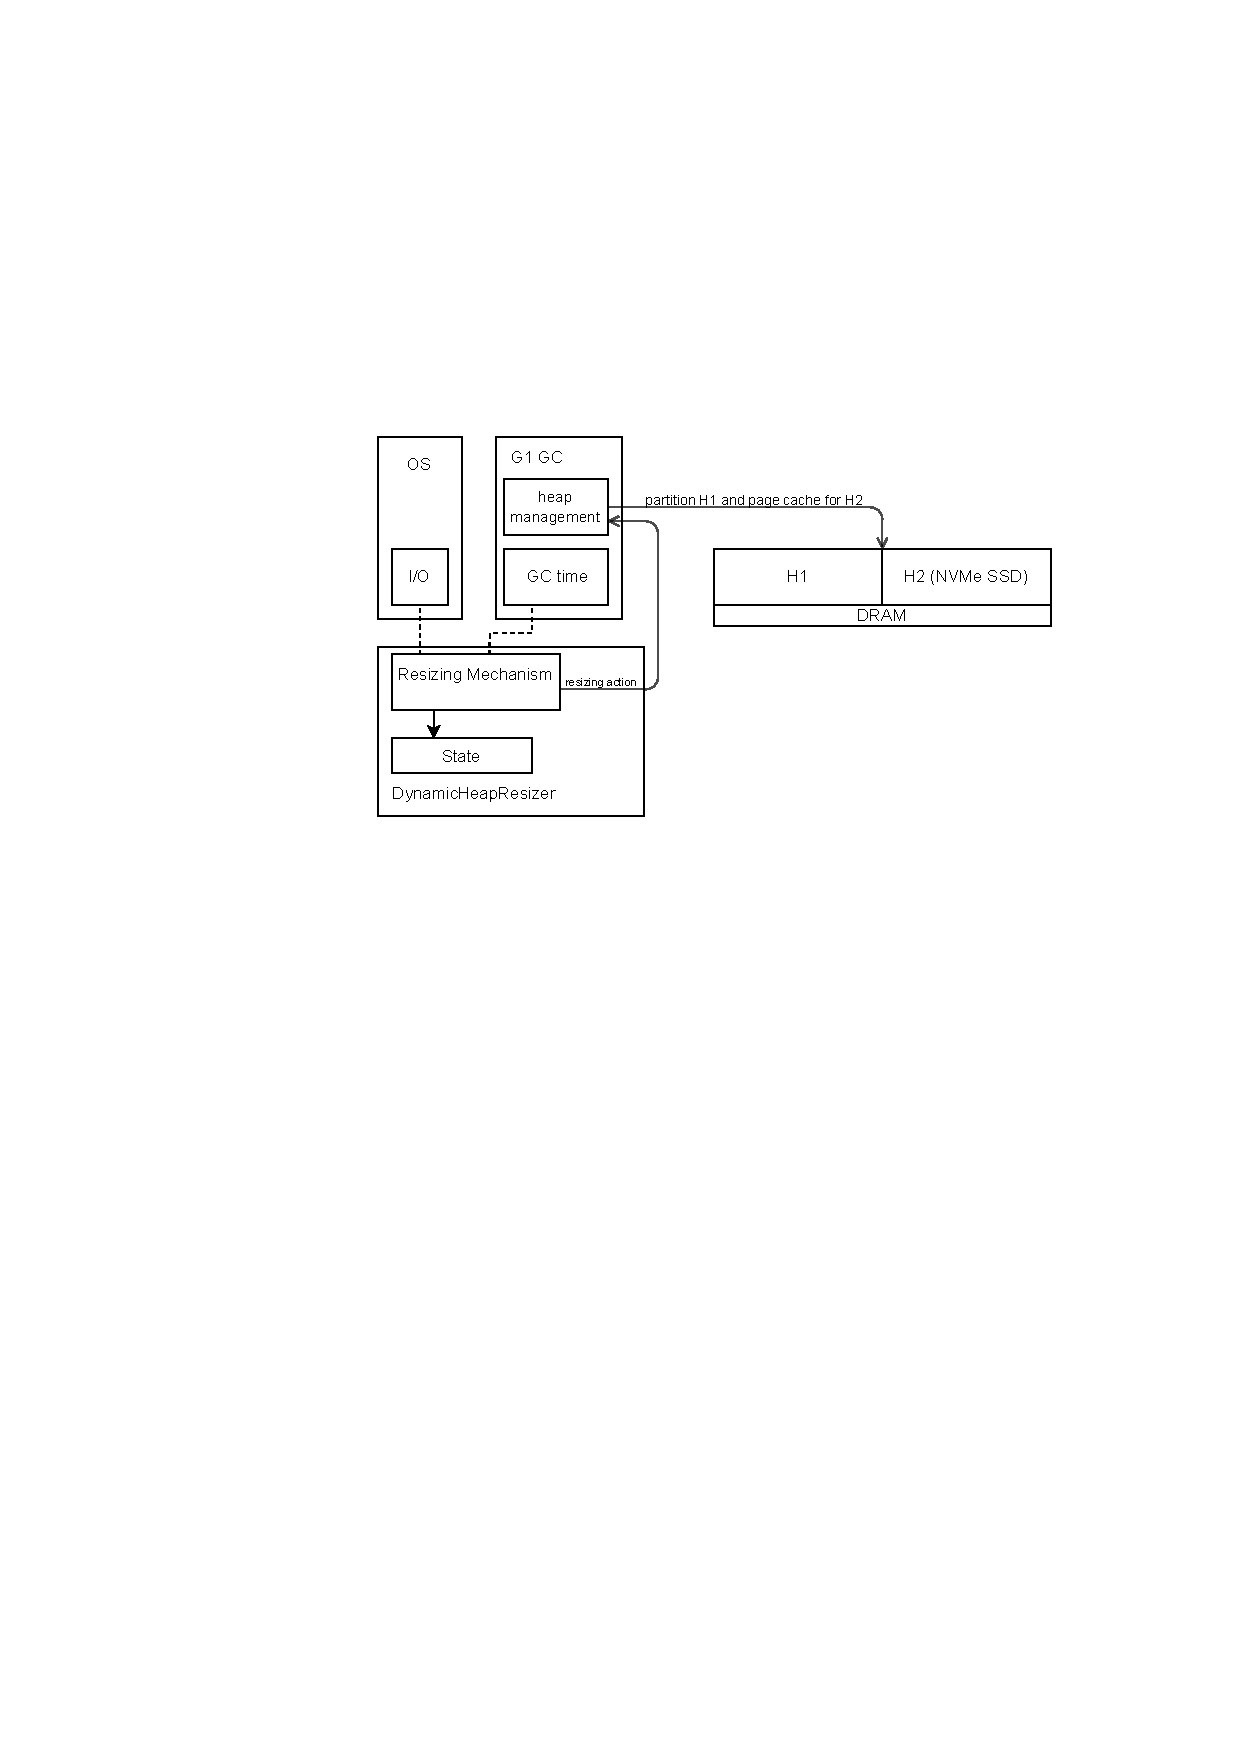
\includegraphics[width=\columnwidth]{fig/HeapResizer.pdf}
  \caption{Overview of the Dynamic Heap Resizer architecture and workflow.}
  \label{fig:dynamic_heap_resizer}
\end{figure}

\subsection{GC overheads}
The Dynamic Heap Resizer operates based on the total compute cycles lost to garbage collection (GC) versus I/O delays to determine how to partition DRAM between the primary managed heap (H1) and the page cache used for the secondary heap (H2). By dynamically resizing H1 at runtime, the system seeks to minimize overall application stall time. To understand this trade-off, we analyze the two key overhead components:
\begin{itemize}
\item \textbf{Stop-The-World (STW) Pauses:}
STW pauses occur when the garbage collector halts all mutator threads to perform marking, evacuation, or compaction tasks. In G1GC, these pauses are triggered by allocation failures or periodic collection cycles. Longer STW pauses directly impact tail latency and user-facing performance, especially for latency-sensitive workloads like Lucene queries.

\item \textbf{Concurrent GC Threads:}
% G1GC employs multiple concurrent GC threads to perform background tasks such as concurrent marking, remembered set rebuilding, and cleanup phases. Although concurrent threads reduce the reliance on long STW pauses, they consume CPU resources that would otherwise be available for application threads. Excessive concurrent GC thread utilization can lead to CPU contention, reducing effective throughput.
The performance impact of these threads depends on CPU allocation and workload conditions. When the total number of mutator and GC threads exceeds the available physical cores (\textit{oversubscription}), GC threads compete with mutators for CPU time, increasing lost compute cycles due to context switching. Under full utilization (when mutator + GC threads equal the number of cores), GC threads do not directly preempt mutators, but still occupy cores that could have been available for additional mutator work. In partial competition scenarios (where the number of threads slightly exceeds the core count), a subset of GC threads preempt mutators, causing partial performance degradation.

\item \textbf{Refinement Threads:}
Refinement threads in G1 process write barriers and maintain the remembered sets required for incremental collection. These threads process card table updates asynchronously to reduce mutator overheads. However, high allocation or mutation rates (e.g. frequent index updates in Lucene) can overload refinement threads, leading to increased CPU utilization or buffer overflow stalls if write barrier queues become saturated.
\end{itemize}

Overall, GC overheads manifest as a combination of direct latency (pause times) and indirect CPU overhead (concurrent and refinement thread activity), both of which reduce application performance.

\subsection{I/O Costs}
The dynamic heap resizer evaluates I/O costs within sampling intervals between GC cycles. Minor GC cycles occur frequently in memory-intensive applications such as Lucene, making them natural boundaries for performance assessment.

To measure I/O cost accurately, we deploy an eBPF hook inside the Linux kernel that records the CPU iowait time by each mutator thread individually. This approach enables us to precisely measure each thread's non-GC/application work. At the end of each sampling interval, these exclusive per-thread iowait measurements are aggregated to calculate the total I/O cost for that interval.

While it is also possible to count major page faults directly, such counts fail to represent true I/O overhead because page fault durations vary significantly, depending on SSD latency, queue depth, and caching state. In contrast, time-based per-thread iowait captures the direct impact of storage delays on application progress.

This unified and precise I/O cost metric is used alongside GC cost estimates to inform resizing decisions, enabling the system to balance H1 heap size against page cache capacity effectively, thereby minimizing overall stall time experienced by mutator threads.


\begin{figure*}[t]
  \centering
  \includegraphics[width=\textwidth]{fig/intervals.pdf}
  \caption{Interval variations for calculating GC cost.}
  \label{fig:intervals}
\end{figure*}

\subsection{Interval variations to calculate GC time}
Figure~\ref{fig:intervals} presents three interval patterns observed in G1GC, presenting how its design combines concurrent phases with stop-the-world pauses to manage memory efficiently \cite{Detlefs2004GarbageFirst}. These patterns highlight the interplay between mutator threads, concurrent GC threads, and refinement threads during different phases of garbage collection, each exhibiting distinct GC cost characteristics relevant to the dynamic heap resizer.

\textbf{(a) Simple GC Interval.} In this pattern, the entire GC time consists solely of a stop-the-world (STW) pause. This occurs when the GC cycle completes within the STW phase without involving any concurrent GC threads. Thus, GC overhead here equals the STW pause duration. 
\begin{equation}
GC_{\text{time}} = STW_{\text{pause}}
\end{equation}
\textbf{(b) Normal Concurrent Mark Cycle.} This interval includes both an STW pause and a concurrent marking phase (CMC). During the concurrent mark, concurrent GC threads traverse the object graph while mutator threads continue executing, while refinement threads process remembered set updates. The interval ends with the STW Remark and Cleanup phases. Therefore, total GC time here is the sum of the concurrent mark duration and the final STW pause.
\begin{equation}
GC_{\text{time}} = CMC + STW_{\text{pause}}
\end{equation}
\textbf{(c) Interrupted Concurrent Mark Cycle.} In this more complex pattern, GC time spans an initial concurrent marking phase (CMC1), followed by an STW pause that interrupts it, and then resumes with a second concurrent marking phase (CMC2). This scenario occurs when an additional GC trigger happens during an ongoing mark cycle, forcing a STW pause. As a result, GC time here is the cumulative duration of CMC1, the STW pause, and CMC2.
\begin{equation}
  GC_{\text{time}} = CMC_{\text{1}} + STW_{\text{pause}} + CMC_{\text{2}}
\end{equation}

These interval variations illustrate different GC scenarios that are compared against I/O costs, enabling the FSM to make informed decisions about resizing the heap accordingly.

\subsection{Decision Making via FSM}

The dynamic heap resizer implements a Finite State Machine (FSM)  as shown in figure \ref{fig:fsm} with three core states to make runtime decisions about growing or shrinking the primary heap (H1). Each state evaluates current GC and I/O metrics to determine the next resizing action, ensuring responsiveness to application memory and I/O demands.

\textbf{1. State: S WAIT GROW.} 
In the S WAIT GROW state, the dynamic heap resizer evaluates the effectiveness of a previous grow action to determine whether further heap expansion is beneficial. Upon entering this state, the system compares the current total lost compute cycles and I/O costs to the delay recorded in the previous interval. If the lost compute cycles have not decreased, this indicates that increasing the heap size did not improve performance. Consequently, the finite state machine transitions to the S WAIT SHRINK state and issues a shrink action to reduce the size of H1, freeing DRAM for the H2 page cache. Conversely, if the lost compute cycles have decreased, the resizer checks the current heap occupancy. When the occupancy is high (exceeding 70\%) and the heap has not reached its maximum allowed size, it remains in S WAIT GROW, issuing another grow action to further expand H1. If occupancy is low, it stays in S WAIT GROW but issues a wait action, pausing further resizing decisions until the next evaluation interval. Overall, this state ensures that heap growth is only reinforced when it yields a measurable reduction in lost compute cycles, maintaining a balance between garbage collection efficiency and available page cache capacity.

\textbf{2. State: S WAIT SHRINK.} 
In the S WAIT SHRINK state, the dynamic heap resizer evaluates the impact of a previous shrink action to determine whether a further heap reduction is required. Upon entering this state, it compares the current total lost compute cycles (GC and I/O costs) to the previously recorded delay. If the lost compute cycles have not decreased, indicating that shrinking H1 did not improve performance, the finite state machine transitions to the S WAIT GROW state and issues a grow action to increase the heap size, aiming to reduce GC overhead by partitioning more DRAM to H1. If the lost compute cycles have decreased, the resizer evaluates system memory slackness by checking whether the combined DRAM usage of the heap and page cache remains below 80\% of the configured DRAM limit. If sufficient slack exists, it remains in S WAIT SHRINK, issuing an IOSLACK action to acknowledge available memory without invoking a resizing action. Otherwise, if slack is limited, the state remains in S WAIT SHRINK but issues an additional shrink action to continue freeing DRAM for the H2 page cache.

\textbf{3. State: S NOACTION.}
In the S NO ACTION state, the dynamic heap resizer maintains its current heap configuration while continuously monitoring system performance. Upon entering this state, it compares the current total lost compute cycles, calculated as the combined GC and I/O costs, to the delay recorded before the last resizing action. If the lost compute cycles have decreased, indicating that the system performance has improved or remained stable without further resizing, the FSM remains in S NO ACTION, issuing no additional actions and preserving the current heap allocation. However, if the lost compute cycles have not decreased, suggesting that the current allocation is suboptimal, the resizer examines the last action executed. If the previous action was a heap shrink and the current heap size has not reached its configured maximum limit, the system transitions to S WAIT GROW and issues a grow action to increase H1, targeting reduced GC overhead. Conversely, if the last action was a grow, the FSM transitions to S WAIT SHRINK and issues a shrink action to reclaim DRAM for the page cache, aiming to reduce I/O costs. If neither condition is met, the FSM remains in S NO ACTION without issuing any resizing commands.

\vspace{0.2cm}

\begin{figure}[htbp]
  \centering
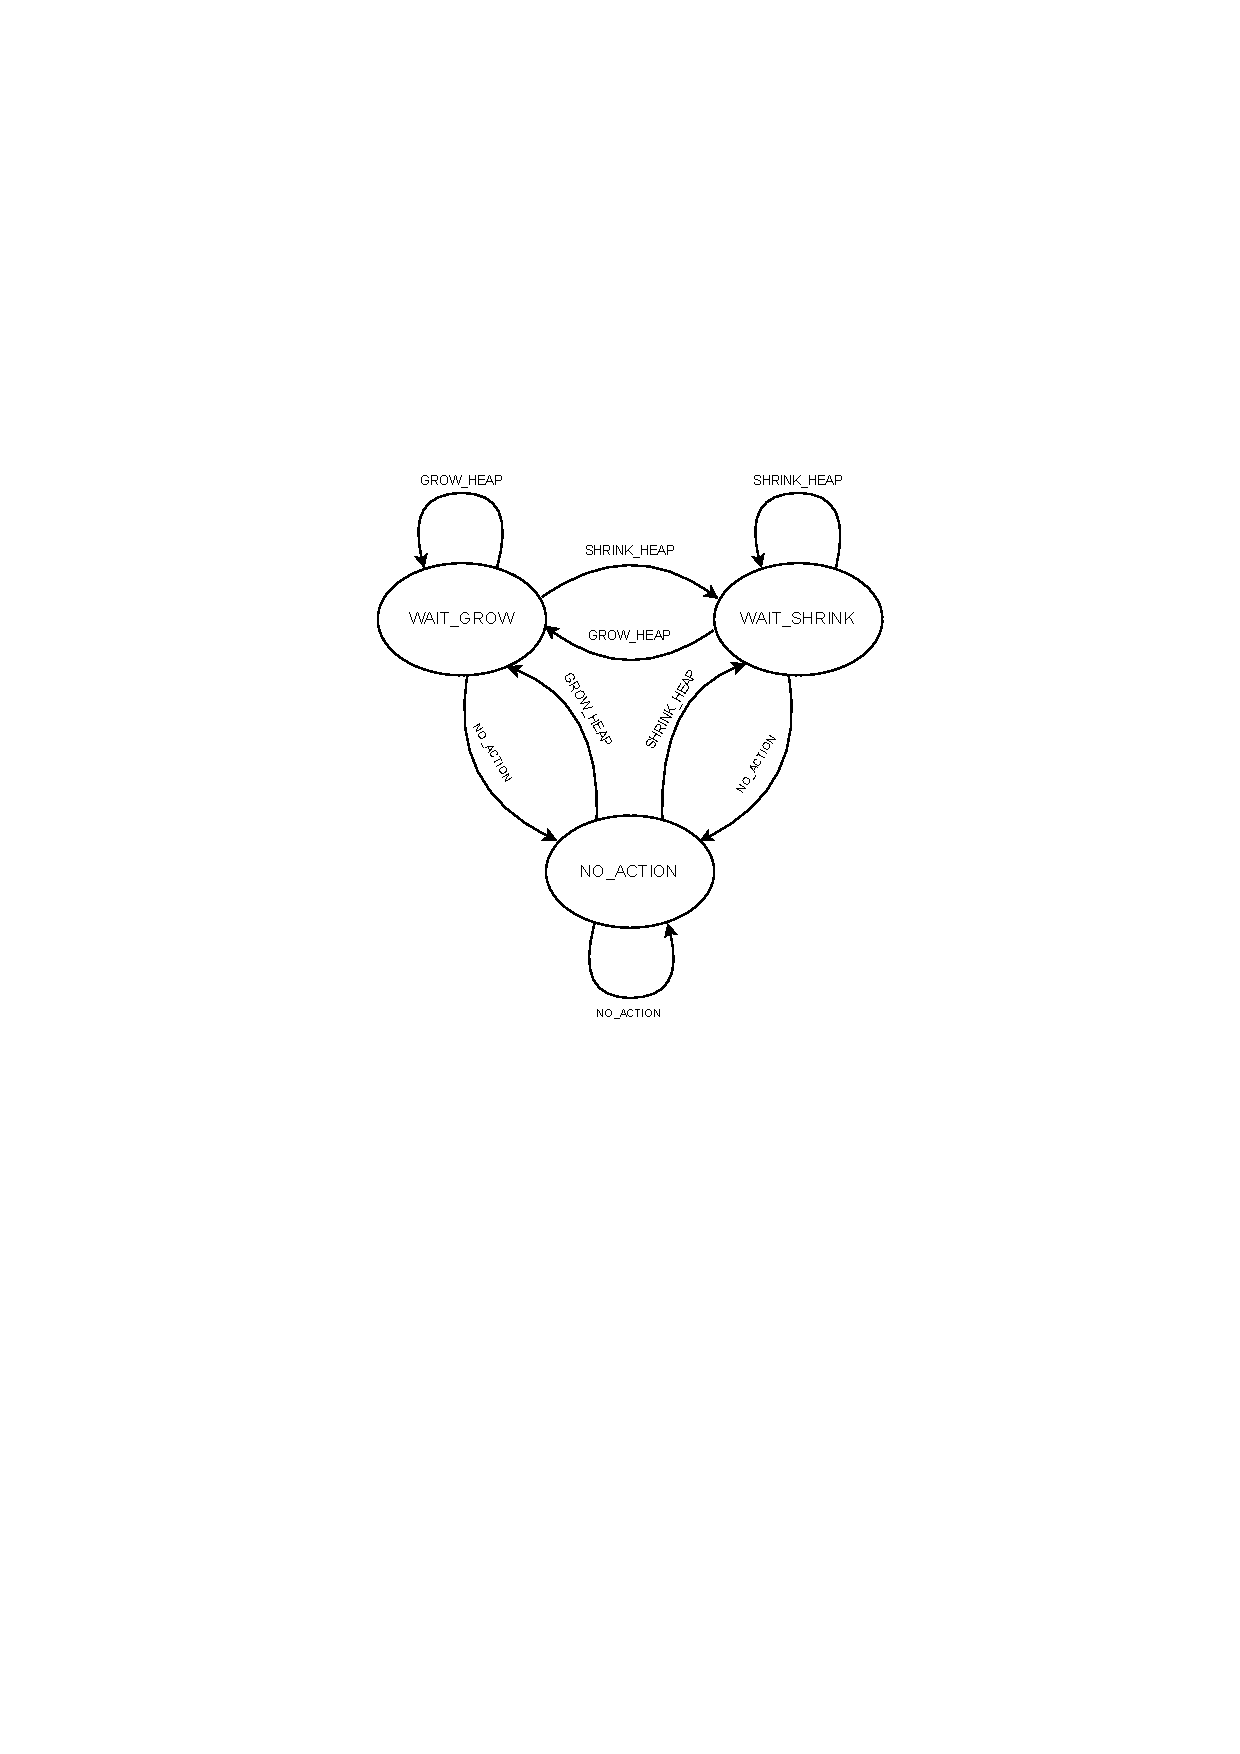
\includegraphics[width=1.1\columnwidth]{fig/FSM.pdf}
  \caption{FSM for heap resizing decisions}
  \label{fig:fsm}
\end{figure}

